\paragraph{The leading-order $\cGW$.}
Under the assumed law~\eqref{eq:cGW}, a positive susceptibility
and physical reference speed $c>0$ give $\cGW>0$.
For every $c\ne0$, the relative speed deviation is
\[
  \dccap(\chivest)
  \equiv \frac{\cGW(\chivest)-c}{c}
  = \sqrt{\chivest}-1.
\]
On the nonnegative domain this deviation is strictly increasing
and vanishes if and only if $\chivest=1$. Thus unity is the exactly
luminal anchor; finite-tolerance compatibility requires an interval
rather than this single value.

\paragraph{Finite-tolerance compatibility.}
Fix $\tau=3\times10^{-15}$ and write
$\verb|LigoSatisfied|(\delta)\equiv|\delta|\leq\tau$
for the conservative symmetric cap.

\begin{theorem}[\texttt{c\_GW\_match\_iff\_chi\_close\_to\_one}]
  \label{thm:bicond}
  For $\chivest\geq0$,
  $\verb|LigoSatisfied|(\dccap(\chivest))
  \;\Longleftrightarrow\;
  \chivest\in[(1-\tau)^2,(1+\tau)^2]$.
\end{theorem}

Indeed, the cap is equivalent to
$1-\tau\leq\sqrt{\chivest}\leq1+\tau$.
Since $0<\tau<1$, both bounds are nonnegative, so squaring
gives the stated interval. Conversely, monotonicity of the
square root recovers the cap from these squared bounds.

Every compatible susceptibility therefore satisfies
\[
  0.1<(1-\tau)^2\leq\chivest\leq(1+\tau)^2<10.
\]
It contains $\chivest=1$ and has nonzero width exactly
$(1+\tau)^2-(1-\tau)^2=4\tau=1.2\times10^{-14}$.
The adopted range has width $9.9$, and the strict comparison is
\[
  10^{14}\bigl[(1+\tau)^2-(1-\tau)^2\bigr]<9.9.
\]
This is a comparison of interval widths within an adopted domain.
It supplies no probability without a prior: under a uniform prior
on $[0.1,10]$, the compatible interval has probability mass
$4\tau/9.9$.

\paragraph{Endpoint checks.}
The endpoints provide quantitative checks of the confinement.

\begin{theorem}[\texttt{natural\_lower\_violates\_ligo}]
  \label{thm:falsifier-lower}
  At $\chivest=0.1$, $\dccap=\sqrt{0.1}-1\approx-0.6838$,
  hence $|\dccap|/\tau\approx2.28\times10^{14}$ and
  \verb|LigoSatisfied| is false.
\end{theorem}

\begin{theorem}[\texttt{natural\_upper\_violates\_ligo}]
  \label{thm:falsifier-upper}
  At $\chivest=10$, $\dccap=\sqrt{10}-1\approx+2.1623$,
  hence $|\dccap|/\tau\approx7.21\times10^{14}$ and
  \verb|LigoSatisfied| is false.
\end{theorem}

The exclusions already follow from
$\sqrt{1/10}\leq\sqrt{1/4}=1/2$ and
$\sqrt{10}\geq\sqrt{4}=2$.
Both endpoints therefore fail simultaneously, while the finite
interval in Theorem~\ref{thm:bicond} remains compatible.
Figure~\ref{fig:cGW} shows this distinction.

\begin{figure}[t]
  \centering
  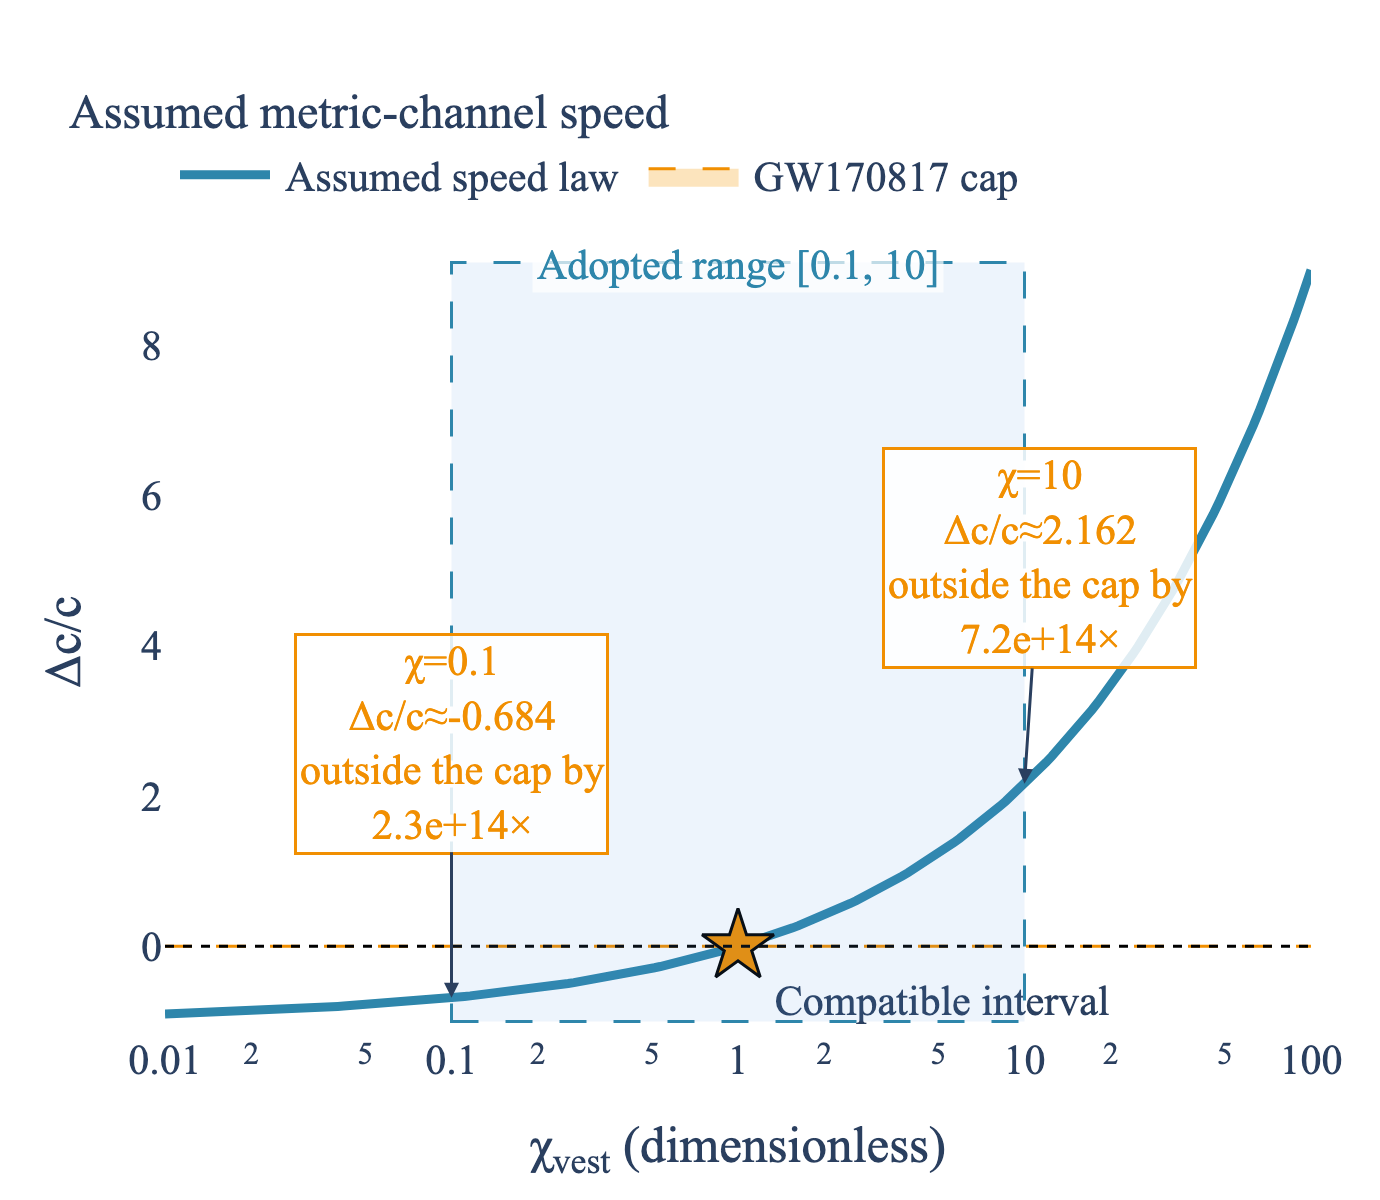
\includegraphics[width=0.96\columnwidth]{figures/fig_c_GW_vs_ligo_constraint.png}
  \caption{\textbf{Headline result.} The
  $\dccap = \sqrt{\chivest} - 1$ deviation across the natural
  $\chivest \in [0.1,10]$ range (pale blue band, dashed blue border)
  versus the conservative symmetric envelope of the
  GW170817~\cite{Abbott2017GW170817} multi-messenger constraint,
  $|\dccap| \leq 3\times 10^{-15}$ (amber, drawn at $\dccap = 0$ because
  the cap's own width is far below one pixel at this scale). Over the
  natural range $\dccap$ sweeps $[-0.68, +2.16]$, exceeding the cap by
  $\sim 10^{14}\times$ \emph{at the endpoints} (orange callouts) and
  vanishing at $\chivest = 1$. The compatible $\chivest$ window
  $[(1-\tau)^2,(1+\tau)^2]$ has width $4\tau = 1.2\times10^{-14}$,
  compared with the adopted range's width $9.9$. Its finite extent is
  unresolved at this scale; the gold star marks its anchor $\chivest=1$,
  not a singleton compatible set. The window sits \emph{inside} the band:
  the datum confines $\chivest$, it does not exclude the range.}
  \label{fig:cGW}
\end{figure}

\paragraph{Compatibility of the identification conditions.}
The proposed identification imposes positivity (P1), compatibility
with the cap (P2), and sub-half-deviation (P3'):
\[
  \begin{aligned}
    &\verb|H_VestigialModeIsGraviton|(\chivest)\\
    &\quad\equiv
      \chivest>0
      \;\wedge\;\verb|LigoSatisfied|(\dccap(\chivest))\\
    &\qquad\wedge\;|\dccap(\chivest)|<1/2.
  \end{aligned}
\]
These three clauses are not independent.
At the fixed tolerance, P2 implies P3' because $\tau<1/2$.
On the nonnegative domain, Theorem~\ref{thm:bicond} also places
every P2-compatible susceptibility in a strictly positive interval,
so P1 holds there. Consequently, the complete compatible set for
these conditions is precisely that same finite interval, including
the anchor $\chivest=1$.

Four counterexamples distinguish compatibility from positivity
alone. The endpoints $0.1$ and $10$ refute the conjunction through
failure of P2. At zero, P1 fails; this point lies outside the
adopted range. At the interior point $\chivest=1/4$,
$\dccap=-1/2$: P1 holds, but P2 and the strict P3' inequality
both fail. The quarter-point example therefore shows that P1
alone does not imply P3'. These counterexamples do not establish
independence of the three clauses or isolate a uniquely failing
clause. The corresponding definitions and algebraic results are
recorded in \texttt{GravitationalWaves.lean}, Sections~1--4.

\paragraph{Endpoint constraints and the open dynamical bridge.}
The endpoint exclusion also applies directly to the relative
deviation of the speed itself:
\[
  \left|\frac{\cGW(\chivest)-c}{c}\right|>\tau,
  \qquad
  \chivest\in\{0.1,10\},\quad c\ne0.
\]
This is the statement of
\texttt{natural\_endpoints\_violate\_ligo\_for\_every\_c};
it includes the physical domain $c>0$ and follows from the
relative-deviation identity above. Changing $c$ therefore
cannot make either endpoint compatible under the assumed law.
This two-point exclusion leaves the compatible interior interval
intact. Neither it nor the $c$-free endpoint statement quantifies
over microscopic actions, propagators or matter couplings, so
neither establishes the absence or impossibility of a dynamical
derivation. A physical application still requires the response
normalization and domain, the physical state, a propagating
tensor mode relative to the same matter/light reference, and
controlled transport and frequency matching with units and
error bounds.

%% ================================================================
